\Chapter{Inleiding}

 In dit inleidende hoofdstuk zal enige achtergrond informatie verschaft worden omtrend cryptografie. Verder zal het concept van identiteits-gebaseerde cryptografie duidelijk gemaakt worden. Er zal uitgelegd worden waarom de recente ondekking van pairings hier zo belangrijk voor is. Ten slotte zal een kort overzicht gegeven worden van in de literatuur terug te vinden implementaties van pairings. In het volgende hoofdstuk wordt de werking van pairings dan wiskundig uitgespit.
\section{Basisachtergrond cryptografie}

Sinds het begin der tijden is er een nood geweest aan manieren om berichten versleuteld te verzenden tussen twee partijen. Voorbeelden van enkele klassieke encryptiemethoden zijn het Atbashcijfer~\cite{athbash} (Babyloni\"e, 600 v.\ Chr.), het Caesarcijfer~\cite{caesar} (Rome, 56 n.\ Chr.) en het dubbele transpositie cijfer~\cite{kahn} (oa.\ gebruikt door weerstandsgroepen in WO II). E\'en eigenschap die al deze methodes met elkaar gemeen hebben, is het gebruik dezelfde sleutel voor versleutelen en ontcijferen. Ook door vele moderne encryptiemethodes, zoals bijvoorbeeld 3DES~\cite{3des} en AES~\cite{aes}, gebruiken dit principe. Dit principe noemt men symetrische versleuteling.

De algemene werking van symetrische cryptografie is weergegeven in \reffig{fig-encryptie-applicaties-sym-cipher}. Alice zendt een bericht $B$ naar Bob door het te versleutelen, vercijferd met een door hen beiden gekende sleutel $k$. Bob op zijn beurt ontcijfert met diezelfde sleutel het bericht. Indien Eve de vooraf afgesproken sleutel kent, kan zij alle communicatie tussen Alice en Bob ontcijferen. Er is dus nood aan een manier om veilig een sleutel $k$ te kunnen afspreken tussen twee partijen.

\begin{figure}[h]
	\centering
		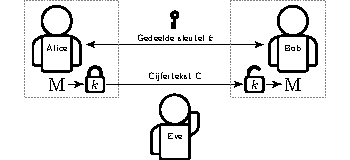
\includegraphics[width=7cm]{symmetric-cipher-model}
		\caption{Algemene werking van symmetrische cryptografie\label{fig-encryptie-applicaties-sym-cipher}}
\end{figure}

Een oplossing voor het veilig afspreken van een gedeelde sleutel was tot 1976 niet gekend. Toen stelden Diffie en Hellman hun algoritme voor sleutel uitwisseling over een onbeveiligd kanaal \cite{diffie-hellman}. Deze ontdekking plaveide de weg voor assymetrische cryptografie (ook wel publieke sleutel cryptografie genoemd). De algemene werking van dit type cryptografie wordt ge\"illustreerd in \reffig{fig-encryptie-applicaties-asym-cipher}. Wanneer Bob een bericht naar Alice wil versturen, zoekt hij eerst haar publieke sleutel op in een databank. Vervolgens versleutelt hij zijn bericht met Alices publieke sleutel. Enkel Alice kan met behulp van haar private sleutel dan het bericht ontcijferen.

\begin{figure}[h]
	\centering
		 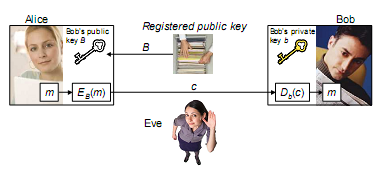
\includegraphics[width=7cm]{asymmetric-cipher-model}
		 \caption{Algemene werking van asymmetrische cryptografie\label{fig-encryptie-applicaties-asym-cipher}}
\end{figure}

Een systeem als dit biedt het grote voordeel dat er geen nood is om de gebruikte (publieke) sleutel geheim te houden. Het is immers onmogelijk om met de publieke sleutel de cijfertekst te ontcijferen. Eve heeft er in dit geval dus geen baat bij de gebruikte publieke sleutel te onderscheppen. 

Om te verzekeren dat de publieke sleutels van elke mogelijk ontvanger voorradig zijn, dient een soort een centrale databank voorzien te worden. Indien iemand het voor anderen mogelijk wil maken hem versleutelde berichten te versturen, genereert die persoon eerst een publieke en private sleutel. De publieke sleutel wordt vervolgens naar de database gestuurd, waar iedereen hem kan ophalen.

% TODO: Meer uitleg? (Wiskunde?)

%Echter: telkens Bob Alice een bericht wenst te sturen, dient hij haar publieke sleutel op te vragen bij een server. Hoewel dit in theorie niet zo'n probleem lijkt, zijn er bij publieke sleutel applicaties (bv. PGP\footnote{Pretty Good Privacy: \url{http://www.prettygoodprivacy.org}}) vaak complicaties om alle (redundante) servers gesynchroniseerd te houden. Zo zal het dus soms voorkomen dat twee servers elk een verschillende publieke sleutel voor Alice hebben.


\section{Identiteits gebaseerde cryptografie}

Een nadeel van de publieke sleutel cryptografie zoals voorgesteld in de vorige paragraaf zit hem in het sleutelbeheer. Er is geen manier om zeker te zijn dat wanneer de publieke sleutel van Alice opgevraagd wordt de verkregen sleutel effectief die van Alice is. Indien Eve bijvoorbeeld haar publieke sleutel in de database laat opslaan onder Alices naam, zal Bob berichten voor Alice versleutelen met Eves publieke sleutel. Een mogelijke oplossing hiervoor is bijvoorbeeld het ``web of trust'', zoals ge\"implementeerd door de software PGP \cite{pgp}. Daarbij kunnen mensen aangeven of ze een bepaalde publieke sleutel betrouwbaar vinden of niet. Een sleutel die vergezeld wordt door meerdere getuigenissen van betrouwbaarheid zal dat dan waarschijnlijk ook zijn. Verder kunnen sleutels opgenomen worden in een zogenaamde ``revocation list'', waardoor wordt aangegeven dat die sleutel niet meer geldig is.

Uiteraard is ook zo een systeem niet volledig waterdicht. Iemand kan bijvoorbeeld onder verschillende identiteiten sleutels insturen en vervolgens met al die verschillende identiteiten zijn sleutels een certificaat van vertrouwen geven. Indien iemands publieke sleutel zou afgeleid kunnen worden van bekende gegevens omtrent zijn identiteit dan zou dit probleem niet bestaan.

In 1984 stelde Shamir een methode voor waarbij dit mogelijk was \cite{shamir}. Het basisidee is als volgt: in plaats van een centrale databank voor publieke sleutels is er een centrale server die private sleutels voor elke gebruiker genereerd aan de hand van geheime parameters. Gebruikers kunnen hun private sleutel dus niet zelf berekenen. De centrale server publiceert ook informatie omtrent hoe iemands identiteitsgegevens kunnen worden omgezet naar een publieke sleutel. Wanneer een gebruiker wil deelnemen aan beveiligde communicatie, meldt hij zich aan bij de centrale server en verkrijgt hij zijn private sleutel alsook de parameters om publieke sleutels te berekenen. Voor zowel de private sleutel als de parameters wordt er van uit gegaan dat deze levenslang gelden. Een gebruiker dient zich dus slechts eenmalig aan te melden.

Uiteraard is ook dit concept niet zonder problemen. Indien bijvoorbeeld de geheime parameters van de centrale server achterhaald worden, is het onmogelijk gebruikers daarvan op de hoogte te brengen. In tegenstelling tot publieke sleutel cryptografie wordt de centrale server nooit gecontacteerd voor een versleuteling en kan dus ook niet met ``revocation lists'' gewerkt worden. Het is dus niet mogelijk bepaalde sleutels (of identiteiten in dit geval) ongeldig te verklaren. Er zijn verschillende oplossingen gepubliceerd voor verscheidene van deze problemen \cite{maas, bla, blie, bloe}. Men kan bijvoorbeeld om de zoveel maanden elke gebruiker nieuwe sleutels bezorgen.

Door deze problemen is identiteits gebaseerde cryptografie eerder geschikt voor kleine groepen mensen, bijvoorbeeld intern in een bedrijf. In dat geval kost het weinig moeite iedereen op regelmatige tijdstippen van nieuwe sleutels te voorzien. 

Hoewel het idee reeds in 1984 gepubliceerd werd, zou het echter tot 2001 duren eer Boneh en Franklin een effici\"ent algoritme voor identiteits-gebaseerde cryptografie zouden voorstellen \cite{boneh}.
